\documentclass[letterpaper,openany,twoside,twocolumn]{book}
%\documentclass[a4paper,openany,oneside,twocolumn]{book}

\newcommand{\PATH}{../../}

\usepackage[justified]{\PATH dndtemplate/dnd}
\usepackage{\PATH monsters/stylesheets/monster_stylesheet}

\usepackage[english]{babel}
\usepackage[utf8]{inputenc}

%\newcommand{\entryfont}{\DndFontStatBlockBody} & uses the default font provided by the LaTeX DnD-Template
\newfontfamily\entryfont{Kalam}[Path=\PATH template/fonts/,Extension=.ttf,UprightFont=Kalam-Regular,BoldFont=Kalam-Bold] % requires XeLaTeX or LuaTeX

\begin{document}

%\layout

\MonsterSheetGeometry

\mainmatter%

% --------------------------------------------------------------------------------------------------- %
% ################################################################################################### %
% #-#-#-#-#-#-#-#-#-#-#-#-#-#-# Monster-Sheet with two Smaller Pictures #-#-#-#-#-#-#-#-#-#-#-#-#-#-# %
% ################################################################################################### %
% --------------------------------------------------------------------------------------------------- %

\MonsterFooterGraphic{0pt}% offset for text to bottom
	{250pt}% max height of the image
	{images/Magma_Turtle_Hatchling.png}% image to be displayed as a banner
	{}% used for keepaspectratio for image ({} or {, keepaspectratio})
	
\nopagebreakchapter{Magma Turtle}

\vspace*{-1.2\fontdimen6\font}

\entryfont \noindent \DndDropCapLine{B}orn of elemental chaos and forged in the crucible of molten earth, the Magma Turtle emerges as a symbol of power and endurance. In its nature, the Magma Turtle maintains a neutral alignment, embodying the harmonious balance between opposing forces. These guardians of the elements exemplify the unbreakable bond between land and water, fire and earth. They stand as reminders of the raw power of nature, shaping and molding life in extraordinary ways. With their presence, they illuminate the delicate balance between fierce determination and graceful adaptation, a testament to the enduring spirit of the Magma Turtle. \\

\paragraph{Species Forms} The creation of these magnificent creatures is a marvel to behold. From humble hatchlings nestled in volcanic rock, their journey begins. The land-dwelling Magma Turtle, absorbing the scorching heat of its volcanic surroundings, grows in stature and resilience. The water-dwelling Magma Turtle, however, undergoes a metamorphosis, adapting to the depths near underwater volcanoes. It becomes reliant on the heat of the surrounding volcanic water, a lifeline for its survival.

In its land form, the Magma Turtle commands attention with its colossal presence. Its stone-hard shell, resembling solidified lava, radiates a fiery glow. With blazing determination in its eyes, it wields a formidable fiery tail club, delivering devastating blows to invaders and attackers. This symbol of power emits licking flames, a warning to those foolish enough to challenge its dominion. Born of fire and stone, the Magma Turtle stands as an indomitable force, ready to unleash its wrath upon any who threaten its realm.

In its water form, the Magma Turtle becomes a majestic ruler of the depths. Its shell, smooth like polished obsidian, reflects the allure of the underwater realm. Fiery luminescence traces sinuous lines on its surface, guiding its path through the watery abyss. With scalding streams of water gushing from its mouth, it repels invaders and attackers, defending its serene aquatic sanctuary. The Magma Turtle, embodying the convergence of fire and water, is a breathtaking sight beneath the waves, showcasing the boundless power and beauty that dwell in the depths.

\vfill\eject % cammand to break to next column

\vspace*{-7.8\fontdimen6\font}
% Monster stat block
\begin{DndMonster}[width=0.5\textwidth]{Magma Turtle (Hatchling)}
    \DndMonsterType{Tiny Elemental, neutral}

    % If you want to use commas in the key values, enclose the values in braces.
    \DndMonsterBasics[
        armor-class = {14 (natural armor)},
        hit-points  = {\DndDice{4d4 + 8}},
        speed       = {20 ft.},
    ]

    \DndMonsterAbilityScores[
        str = 8,
        dex = 13,
        con = 15,
        int = 2,
        wis = 12,
        cha = 7,
    ]

    \DndMonsterDetails[
        saving-throws = {Con +4},
        %skills = {Acrobatics +0, Animal Handling +0, Arcana +0, Athletics +0, Deception +0, History +0, Insight +0, Intimidation +0, Investigation +0, Medicine +0, Nature +0, Perception +0, Performance +0, Persuasion +0, Religion +0, Sleight of Hand +0, Stealth +0, Survival +0},
        damage-vulnerabilities = {cold},
        damage-resistances = {Bludgeoning, Piercing, and Slashing from Nonmagical Attacks},
        damage-immunities = {Fire},
        senses = {Darkvision 60ft., Passive Perception 11},
        condition-immunities = {Exhaustion, Paralyzed, Petrified, Poisoned},
        languages = {understands Primordial but can't speak},
        challenge = 1/2,
    ]
    
    \DndMonsterAction{Fire Vulnerability}
    For every 5ft. the Magma Turtle (Hatchling) moves through water or for each each gallon of water splashed on it, it takes 1 cold damage.
    
    \DndMonsterAction{Molten Rock Shell}
    The Magma Turtle's (Hatchling) shell provides it with resistance to bludgeoning, piercing, and slashing damage from nonmagical attacks.
	
	\DndMonsterSection{Actions}
	
	\DndMonsterAttack[
      name=Bite,
      distance=melee, % valid options are in the set {both,melee,ranged},
      %type=weapon, %valid options are in the set {weapon,spell}
      mod=+1,
      reach=5,
      %range=20/60,
      targets=one target,
      dmg=\DndDice{1d4 + 1},
      dmg-type=piercing,
      %plus-dmg=,
      %plus-dmg-type=,
      %or-dmg=,
      %or-dmg-when=,
      %extra=,
    ]
    
    \DndMonsterSection{Reactions}
    
    \DndMonsterAction{Shell Defense}
    When the Magma Turtle (Hatchling) is hit by a melee attack, it can use its reaction to retract into its shell, gaining a +2 bonus to its AC until the start of its next turn.
      
\end{DndMonster}

\paragraph{Magma Turtle (Hatchling)}
A mesmerizing creature, embodying the essence of fire and stone. A small marvel, its robust, stone-hard shell resembles solidified lava. Adorned with intricate, glowing cracks, it emits vibrant red light, casting an otherworldly radiance. Agile and resilient, it scampers with grace near underwater volcanoes, absorbing intense heat. Fiery eyes shimmer with determination, vigilant for threats and warmth.

Its compact frame and formidable shell hint at future power. Each day, it grows stronger, harnessing volcanic energy. On the cusp of transformation, the hatchling will become a mighty Magma Turtle. In its presence, one feels latent power and untamed potential. This captivating \blocktextlinebreak\hspace*{1cm}hatchling will emerge, a force to reckon with, \blocktextlinebreak\hspace*{3cm}navigating land and water, unmatched in \blocktextlinebreak\hspace*{5.5cm}strength and endurance.

\newpage

\MonsterFooterGraphic{50pt}% offset for text to bottom
	{300pt}% max height of the image
	{images/Magma_Fields.png}% image to be displayed as a banner
	{}% used for keepaspectratio for image ({} or {, keepaspectratio})

\begin{tikzpicture}[overlay, remember picture, inner sep=0pt, outer sep=0pt, path fading=fade down]%
	\node (posN) at (current page text area.north) {};%
	\node[above left=20pt and 5.75cm of posN, anchor=north] (cornerNW) {%
		\begin{minipage}{\columnwidth}%%
        	\centering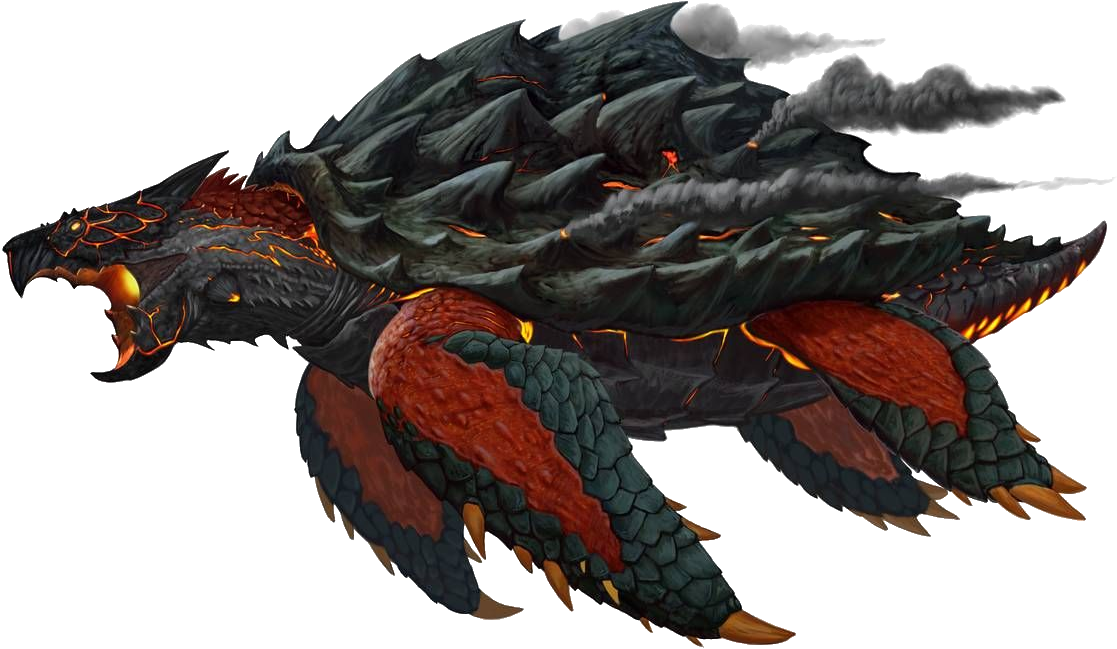
\includegraphics[width=1.1\columnwidth, height=280pt, keepaspectratio]{images/Magma_Turtle_Waterform.png}%
      	\end{minipage}%
	};%
\end{tikzpicture}%

\hfill\\\vspace*{1.75cm}

% Monster stat block
\begin{DndMonster}[width=0.5\textwidth]{Magma ~~~~~~~~~~~~~~ Turtle\\(Waterform)}
    \DndMonsterType{Large Elemental, neutral}

    % If you want to use commas in the key values, enclose the values in braces.
    \DndMonsterBasics[
        armor-class = {18 (natural armor)},
        hit-points  = {\DndDice{12d10 + 60}},
        speed       = {10 ft., 60 ft. swim},
    ]

	\renewcommand{\AbilityScoreSpacer}{~}
    \DndMonsterAbilityScores[
        str = 14,
        dex = 14,
        con = 20,
        int = 6,
        wis = 12,
        cha = 8,
    ]

    \DndMonsterDetails[
        saving-throws = {Dex +4, Con +7},
        skills = {Perception +4},
        %damage-vulnerabilities = {Fire},
        damage-resistances = {Bludgeoning, Piercing, and Slashing from Nonmagical Attacks},
        damage-immunities = {Fire},
        senses = {Darkvision 60ft, Passive Perception 14},
        condition-immunities = {Petrified},
        languages = {Primordial},
        challenge = 7,
    ]
    
	\DndMonsterAction{Amphibious}
	The Magma Turtle (Waterform) can breathe air and water.
	
	\DndMonsterAction{Keen Smell}
	The Magma Turtle (Waterform) has advantage on Wisdom (Perception) checks that rely on smell.
    
    \DndMonsterAction{Scorching Rampage}
    Whenever the Magma Turtle is hit by a fire-based attack, its fiery nature intensifies. On its next successful attack, the Magma Turtle inflicts an additional \DndDice{2d6} fire damage. This increase in damage lasts until the end of its next turn.
	
	\DndMonsterSection{Actions}
	
	\DndMonsterAction{Multiattack}
	The Magma Turtle (Waterform) can make one Pound Attack and one Fiery Stream Attack on each of its turns.
	
	\DndMonsterAttack[
      name=Pound,
      distance=melee, % valid options are in the set {both,melee,ranged},
      %type=weapon, %valid options are in the set {weapon,spell}
      mod=+7,
      reach=5,
      %range=20/60,
      targets=one target,
      dmg=\DndDice{2d8 + 5},
      dmg-type=bludgeoning,
      %plus-dmg=,
      %plus-dmg-type=,
      %or-dmg=,
      %or-dmg-when=,
      %extra=,
    ]
    
    \DndMonsterAction{Fiery Streams}
	The Magma Turtle (Waterform) can unleash hot streams of water as a ranged spell attack (+4 to hit, 20/60 ft. range). All targets in the line of effect must make a DC 15 Dexterity saving throw taking \DndDice{4d8} fire damage on a failed one, or half damage on a successful save.
    
    \DndMonsterSection{Reactions}
    
    \DndMonsterAction{Shell Defense}
    When the Magma Turtle (Waterform) is hit by a melee attack, it can use its reaction to retract into its shell, gaining a +4 bonus to its AC until the start of its next turn.
      
\end{DndMonster}

\vfill\eject % command to break to next column

% Monster stat block
\begin{DndMonster}[width=0.5\textwidth +0.5em]{Magma Turtle (Landform)}
    \DndMonsterType{Large Elemental, neutral}

    % If you want to use commas in the key values, enclose the values in braces.
    \DndMonsterBasics[
        armor-class = {18 (natural armor)},
        hit-points  = {\DndDice{16d10 + 80}},
        speed       = {20 ft.},
    ]

    \DndMonsterAbilityScores[
        str = 20,
        dex = 10,
        con = 20,
        int = 6,
        wis = 12,
        cha = 8,
    ]

    \DndMonsterDetails[
        saving-throws = {Con +9},
        skills = {Athletics +9, Perception +5},
        damage-vulnerabilities = {Cold},
        damage-resistances = {Bludgeoning, Piercing, and Slashing from Nonmagical Attacks},
        damage-immunities = {Fire},
        senses = {Darkvision 60ft, passive Perception 15},
        condition-immunities = {Exhaustion, Paralyzed, Petrified, Poisoned},
        languages = {Primordial},
        challenge = 8,
    ]
    
    \DndMonsterAction{Fire Vulnerability}
    For every 5ft. the Magma Turtle (Landform) moves through water or for each each gallon of water splashed on it, it takes 4 cold damage.
    
    \DndMonsterAction{Scorching Rampage}
    Whenever the Magma Turtle is hit by a fire-based attack, its fiery nature intensifies. On its next successful attack, the Magma Turtle inflicts an additional \DndDice{2d6} fire damage. This increase in damage lasts until the end of its next turn.
	
	\DndMonsterSection{Actions}
	
	\DndMonsterAction{Multiattack}
	The Magma Turtle (Landform) can make one Bite Attack and one Fiery Tail Club Attack on each of its turns.
	
	\DndMonsterAttack[
      name=Bite,
      distance=melee, % valid options are in the set {both,melee,ranged},
      %type=weapon, %valid options are in the set {weapon,spell}
      mod=+9,
      reach=10,
      %range=20/60,
      targets=one target,
      dmg=\DndDice{3d8 + 6},
      dmg-type=piercing,
      %plus-dmg=,
      %plus-dmg-type=,
      %or-dmg=,
      %or-dmg-when=,
      %extra=,
    ]
    
    \DndMonsterAttack[
      name=Fiery Tail Club,
      distance=melee, % valid options are in the set {both,melee,ranged},
      %type=weapon, %valid options are in the set {weapon,spell}
      mod=+9,
      reach=20,
      %range=20/60,
      targets=one target,
      dmg=\DndDice{3d10 + 6},
      dmg-type=bludgeoning,
      plus-dmg=\DndDice{2d6},
      plus-dmg-type=fire,
      %or-dmg=,
      %or-dmg-when=,
      extra={. If the target hit is a creature it must succeed a DC 16 Strength saving throw or be knocked prone},
    ]
    
    \DndMonsterSection{Reactions}
    
    \DndMonsterAction{Shell Defense}\hfill\\
    When the Magma\\Turtle (Landform) is\\hit by a melee attack\\it can use its reaction\\to retract into its shell,\\gaining a +4 bonus to\\its AC until the start of its\\next turn.
      
\end{DndMonster}

\begin{tikzpicture}[overlay, remember picture, inner sep=0pt, outer sep=0pt, path fading=fade down]%
	\node (posN) at (current page text area.north) {};%
	\node[above left=20pt and 5.75cm of posN, anchor=north] (cornerNW) {%
		\begin{minipage}{\columnwidth}%%
        	\centering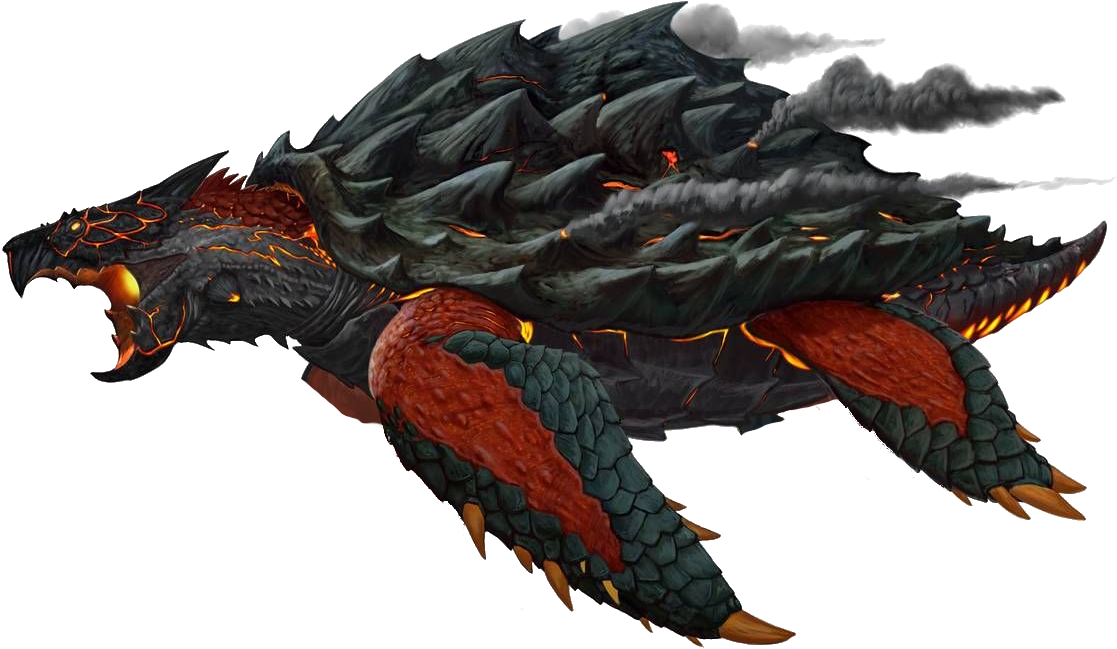
\includegraphics[width=1.1\columnwidth, height=280pt, keepaspectratio]{images/Magma_Turtle_Waterform_above.png}%
      	\end{minipage}%
	};%
\end{tikzpicture}%

\begin{tikzpicture}[overlay, remember picture, inner sep=0pt, outer sep=0pt, path fading=fade down]%
	\node (posS) at (current page text area.south) {};%
	\node[below right=-90pt and 6.85cm of posS, anchor=south] (cornerSE) {%
		\begin{minipage}{\columnwidth}%%
        	\centering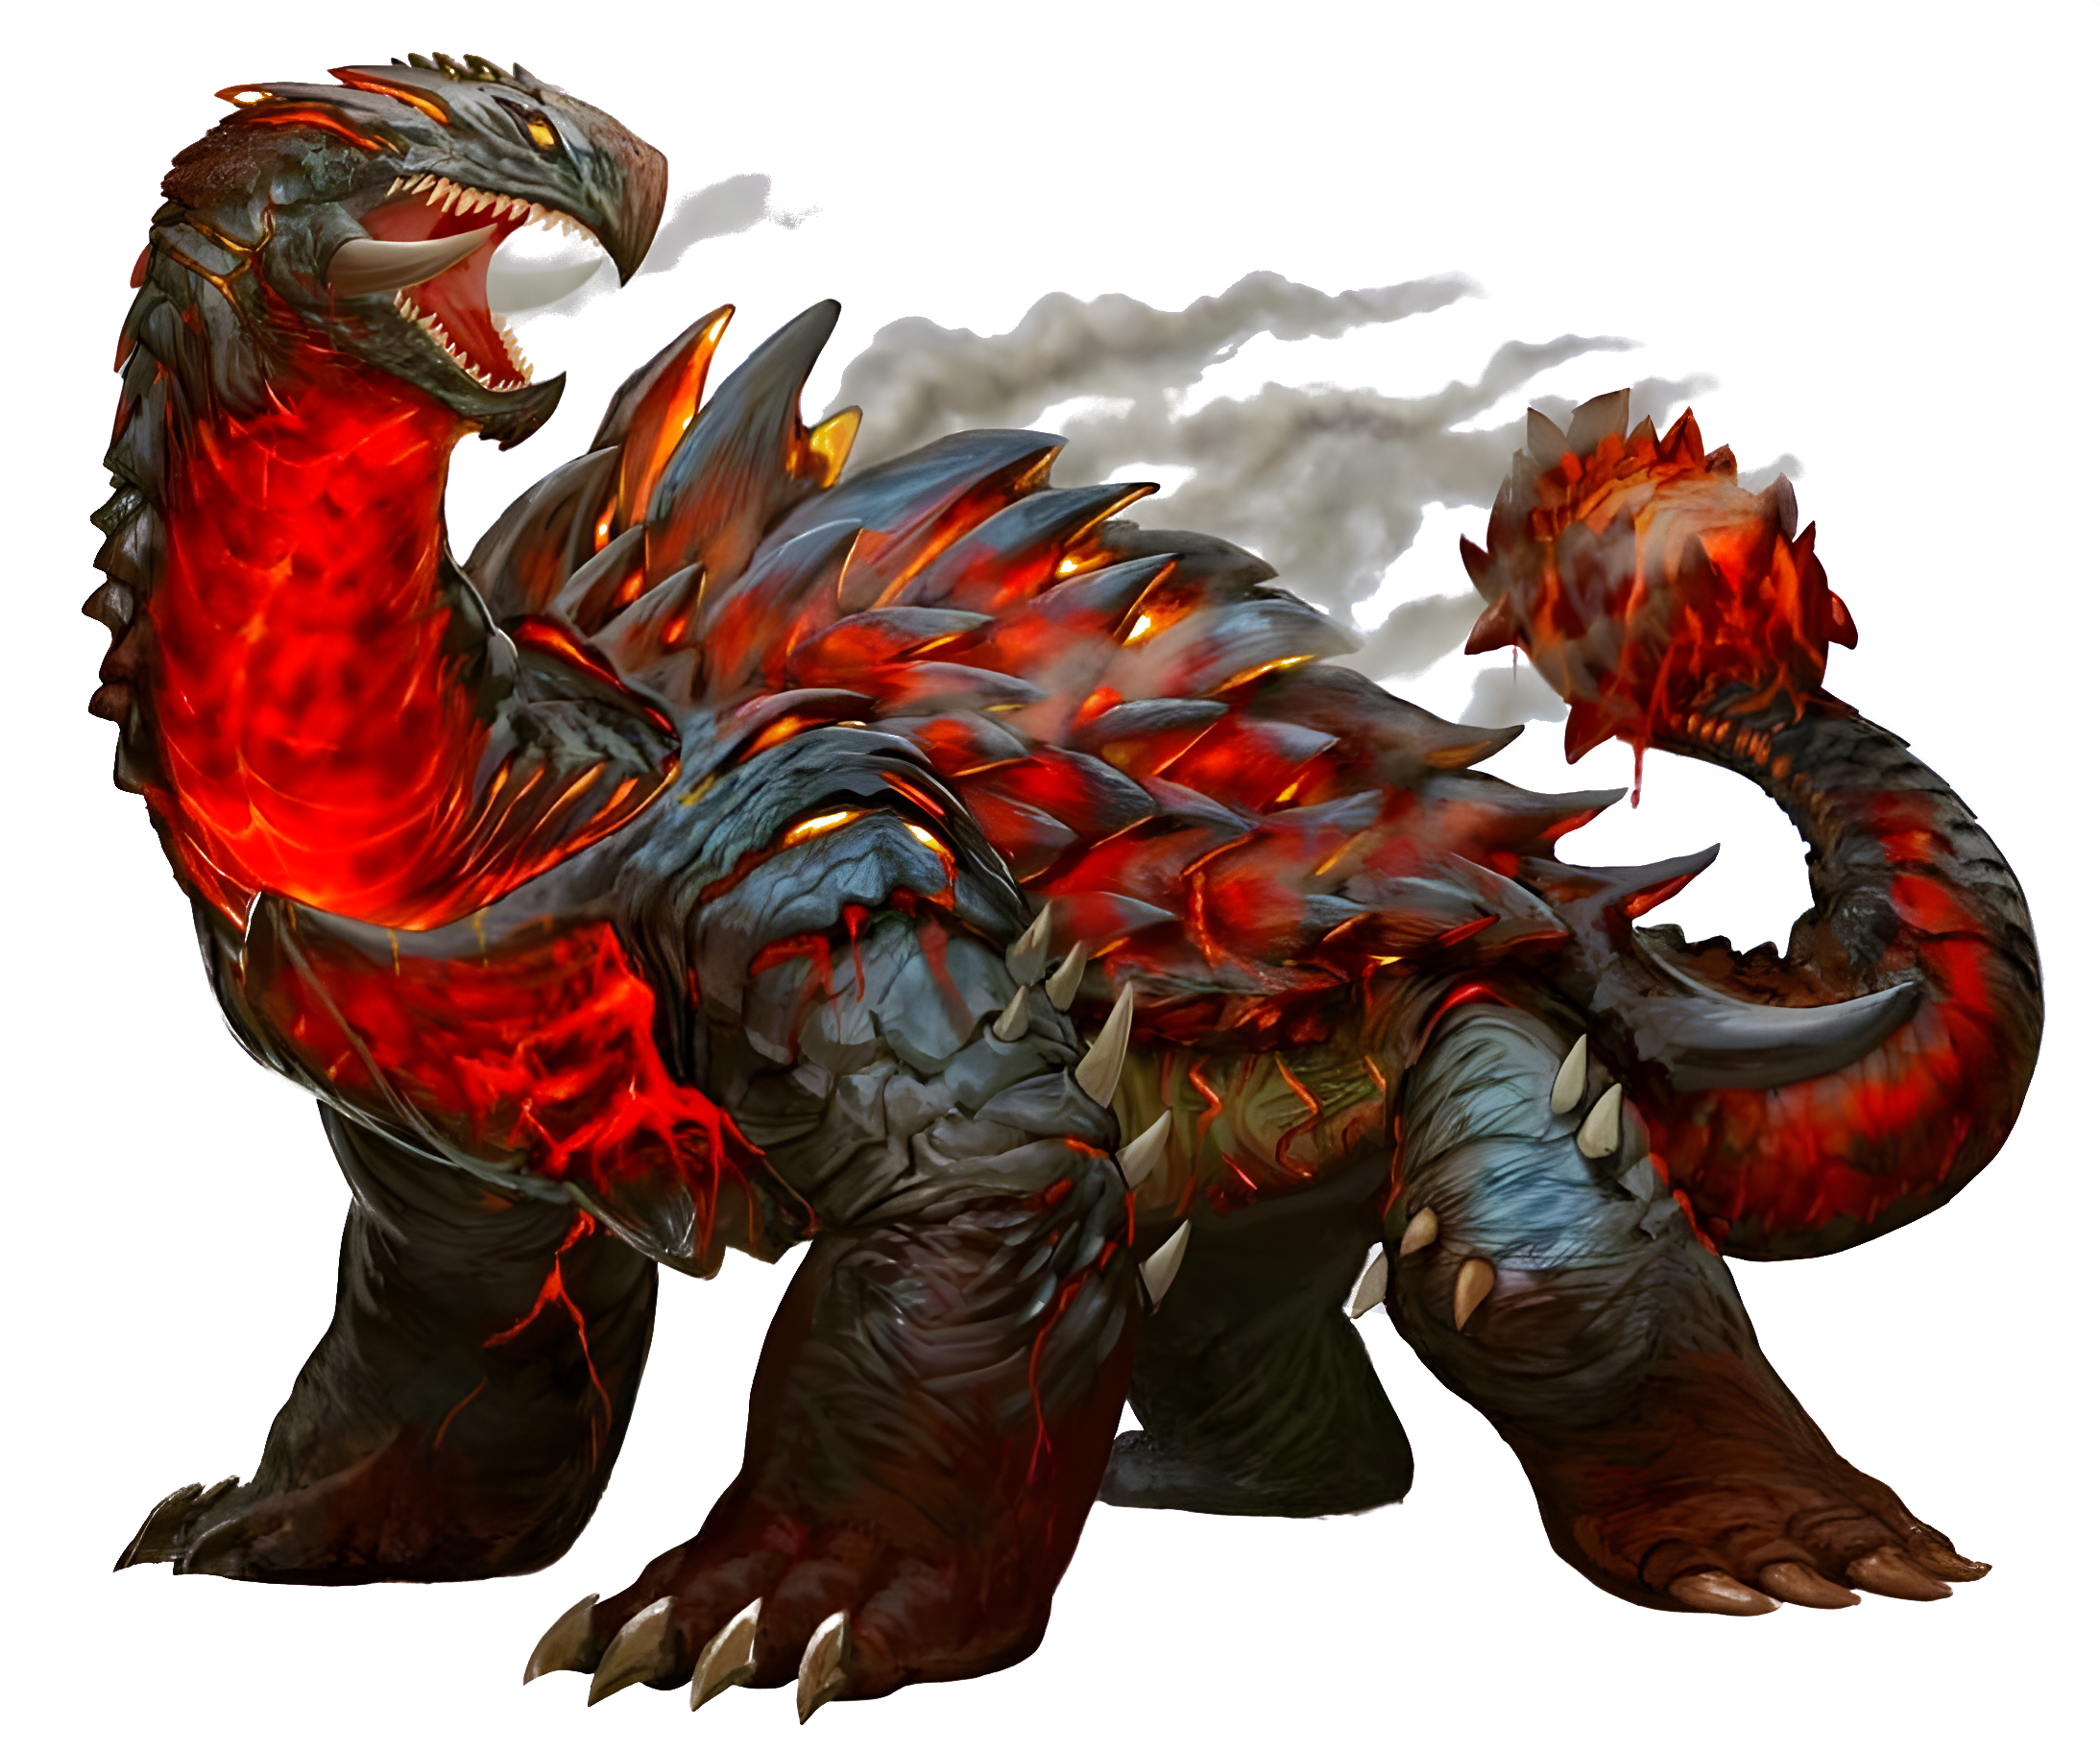
\includegraphics[width=\columnwidth, height=180pt, keepaspectratio]{images/Magma_Turtle_Landform(2).png}%
      	\end{minipage}%
	};%
\end{tikzpicture}%

\end{document}
